\documentclass[10pt,a4paper]{article}
\usepackage[utf8]{inputenc}
\usepackage{amsmath}
\usepackage{amsfonts}
\usepackage{amssymb}
\usepackage{graphicx}

\author{Oleg Loshkin}
\title{\textbf{UPDC}\\Unity to PokEngine Data Converter\\\textbf{User Manual}}
\graphicspath{{./images/}}

\begin{document}
\maketitle
\section{Introduction}
The \textbf{Unity to PokEngine Data Converter, or UPDC for short}, is a Unity tool used to \textbf{export ScriptableObject} inheriting .asset files \textbf{into JSON files} that end with extensions that specify their type. These JSON files can then be read by the PokEngine's parser.

\section{Accessing the Tool}
\begin{figure}[h]
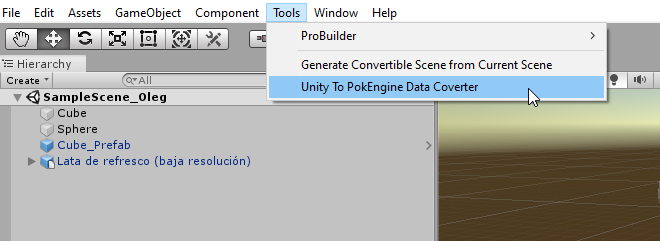
\includegraphics[width=\textwidth]{mainMenu}
\end{figure}
\noindent The tool is accessed via \textbf{MainMenu/Tools/Unity to PokEngine Data Converter}.
\newpage

\section{The Exporter Tab}
\begin{center}
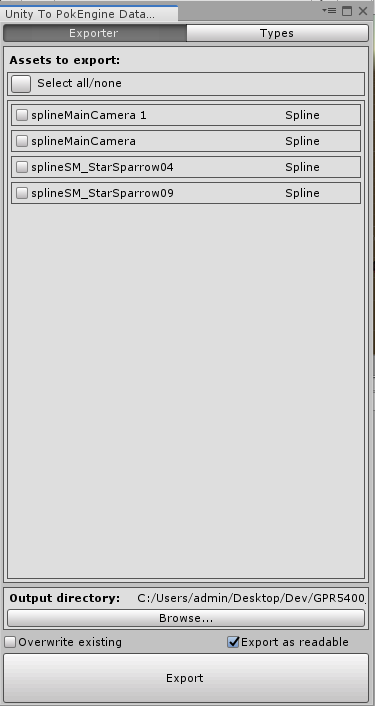
\includegraphics[scale=0.70]{UPDC_UI}
\end{center}
The tool is separated between \textbf{two tabs}. In the \textbf{Exporter tab}, you can \textbf{select the .asset files located in the Assets/Data/...} folders \textbf{you wish to export}.\\
You can \textbf{select the output directory} for the files generated. By default, the tool outputs the files into Assets/Editor/UPDC/DefaultOutputDir.
Upon exportation, \textbf{directories will be generated in the output directory} to mirror the structure seen in Assets/Data.\\
Finally, you can choose to \textbf{overwrite any existing files} and choose between a \textbf{human friendly readable format} or an \textbf{optimised one} for the JSON.
\newpage

\section{Integrating with UPDC}
\textbf{UPDC converts .asset files} of types \textbf{inheriting from the ScriptableObject} class.\\
If you wish to export your data using UPDC, you will therefore need to \textbf{create your ScriptableObject inheriting class} and store instances of it you wish exported in the \textbf{Assets/Data/yourTypeNameHere folder}. \textbf{This must be done on your side}.\\
Next, you will need to \textbf{define your new class with UPDC} via the "Types" tab.

\section{The Types Tab}
The \textbf{Types tab} contains a list of \textbf{tuples that define a type's name and it's corresponding extension}.
The type's name is used for generating appropriately named folders and the extension is appended to the JSONs generated for your custom class to be used by the PokEngine's parser to identify the asset's type.\\
\textbf{To integrate your newly created class} with UPDC, simply \textbf{enter it's name and it's extension} in the "New entry" fields and press the \textbf{"Add new type" button}.
\begin{center}
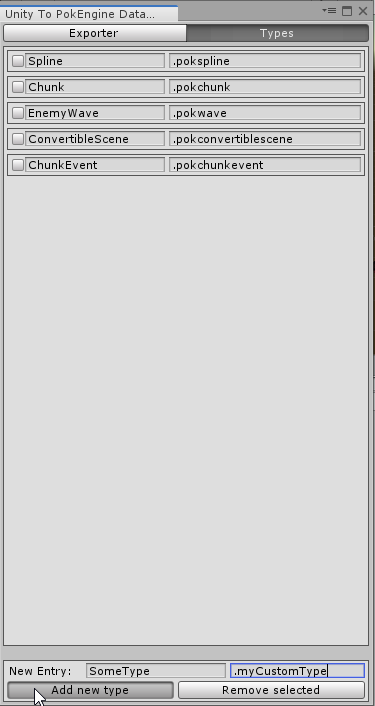
\includegraphics[scale=0.60]{addingType}
\end{center}
\newpage
\noindent A \textbf{folder for your new .asset files will be automatically generated} in Assets/Data and the files will be visible in the "Export" tab.\\
To \textbf{remove a type}, simply \textbf{select it} in the list and press the \textbf{"Remove selected" button}.
\begin{center}
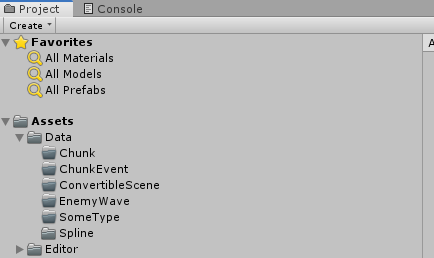
\includegraphics[scale=1.0]{dataFolder}
\end{center}

TODO: comment on images, pic of a ScriptableObject code to integrate

\end{document}
